\documentclass[12pt]{article}
\usepackage[paperwidth=91.44cm,paperheight=106.68cm,margin=0cm]{geometry}
\usepackage[T1]{fontenc}
\usepackage[utf8]{inputenc}
\usepackage{lmodern}
\usepackage{helvet}
\renewcommand{\familydefault}{\sfdefault}
\usepackage{amsmath,amssymb}
\usepackage{graphicx,xcolor,booktabs,tabularx,array}
\usepackage{ragged2e}
\usepackage{tikz}
\usepackage[most]{tcolorbox}
\usepackage[absolute,overlay]{textpos}
\usepackage{qrcode}
\usepackage[hidelinks]{hyperref}
\hypersetup{pdftitle={AI-Assisted Prioritization of VAERS Signal Candidates},pdfauthor={Natanael Alpay},pdfsubject={Retrospective next-quarter threshold-crossing prediction; corrected training-only imputation}}
\pagestyle{empty}
\setlength{\parindent}{0pt}
\setlength{\parskip}{0pt}
\hyphenpenalty=10000
\exhyphenpenalty=10000
\DeclareMathSizes{30}{30}{21}{16}
\DeclareMathSizes{27}{27}{19}{14}
\setlength{\TPHorizModule}{1cm}
\setlength{\TPVertModule}{1cm}
\textblockorigin{0cm}{0cm}
\definecolor{Navy}{HTML}{082B48}
\definecolor{Blue}{HTML}{17558B}
\definecolor{Teal}{HTML}{008F95}
\definecolor{Gold}{HTML}{EABF58}
\definecolor{Ink}{HTML}{253C50}
\definecolor{Muted}{HTML}{536A7B}
\definecolor{Pale}{HTML}{F1F5F8}
\definecolor{Line}{HTML}{D8E2E9}
\definecolor{Ice}{HTML}{BCD5E5}
\color{Ink}

\newcommand{\bodyfont}{\fontsize{29}{37}\selectfont}
\newcommand{\smallbody}{\fontsize{27}{35}\selectfont}
\newcommand{\captionfont}{\fontsize{27}{35}\selectfont}
\newcommand{\labeltext}[1]{{\color{Blue}\bfseries #1}}
\newcommand{\spacepara}{\par\vspace{0.42cm}}
\newcommand{\bulletline}[1]{\par\noindent\hangindent=0.72cm\hangafter=1{\color{Teal}\textbullet}\hspace{0.35cm}#1\par\vspace{0.22cm}}
\newcommand{\colheading}[3]{%
\begin{textblock*}{28.68cm}(#1cm,18.0cm)
{\fontsize{24}{28}\selectfont\color{Teal}\bfseries #2}\hspace{0.42cm}%
{\fontsize{36}{42}\selectfont\color{Navy}\bfseries #3}
\end{textblock*}}
\newtcolorbox{posterbox}[2]{enhanced,width=\linewidth,height=#1,
  colback=white,colframe=Line,colbacktitle=white,coltitle=Navy,
  boxrule=0.7pt,arc=2.3mm,boxsep=0pt,left=0.85cm,right=0.85cm,
  top=0.35cm,bottom=0.6cm,lefttitle=0.85cm,righttitle=0.85cm,
  toptitle=0.6cm,bottomtitle=0.35cm,titlerule=0pt,
  fonttitle=\fontsize{33}{39}\selectfont\bfseries,fontupper=\bodyfont\RaggedRight,
  before skip=0pt,after skip=0pt,valign=top,breakable=false,
  borderline north={3pt}{0pt}{Blue},title={#2}}
% Auto-generated from corrected result tables.
\newcommand{\TestN}{6,926}
\newcommand{\TestPos}{294}
\newcommand{\BaseRate}{4.24\%}
\newcommand{\ReviewsGB}{806}
\newcommand{\ReviewsBaseline}{1,531}
\newcommand{\Reduction}{47.4\%}
\newcommand{\FewerReviews}{725}
\newcommand{\TopHundred}{32}
\newcommand{\Lift}{7.5}
\newcommand{\GBAP}{0.205}
\newcommand{\CIlo}{0.169}
\newcommand{\CIhi}{0.249}
\newcommand{\NoTemporalAP}{0.119}
\newcommand{\GBEighty}{1,980}
\newcommand{\BaselineEighty}{5,696}
\newcommand{\ReductionEighty}{65.2\%}


\begin{document}
\begin{tikzpicture}[remember picture,overlay]
\fill[Pale] (current page.north west) rectangle (current page.south east);
\fill[Navy] (current page.north west) rectangle ([yshift=-8.25cm]current page.north east);
\fill[Gold] ([yshift=-8.25cm]current page.north west) rectangle ([yshift=-8.36cm]current page.north east);
\fill[white] ([yshift=-103.0cm]current page.north west) rectangle (current page.south east);
\draw[Line,line width=1pt] ([yshift=-103.0cm]current page.north west)--([yshift=-103.0cm]current page.north east);
\end{tikzpicture}

% Original transparent institutional logos, placed without recoloring or stretching.
\begin{textblock*}{15.5cm}(1.6cm,2.6cm)

\includegraphics[width=15.5cm]{branding/uci_physical_sciences.png}
\end{textblock*}
\begin{textblock*}{5.0cm}(84.84cm,1.65cm)

\includegraphics[width=5.0cm]{branding/uci_seal.png}
\end{textblock*}

% Centered header. 36 inches wide by 42 inches tall, preserving the corrected analysis.
\begin{textblock*}{88.24cm}(1.6cm,0.85cm)
\centering
{\fontsize{60}{72}\selectfont\bfseries\color{white}AI-Assisted Prioritization of VAERS Signal Candidates}
\end{textblock*}
\begin{textblock*}{88.24cm}(1.6cm,4.15cm)
\centering
{\fontsize{37}{44}\selectfont\color{Ice}A retrospective study of next-quarter threshold crossings for expert review}
\end{textblock*}
\begin{textblock*}{88.24cm}(1.6cm,6.12cm)
\centering
{\fontsize{32}{39}\selectfont\color{white}\textbf{Natanael Alpay}\hspace{0.75cm}\textcolor{Ice}{|}\hspace{0.75cm}University of California, Irvine}
\end{textblock*}

% A single, spacious findings strip replaces three competing headline boxes.
\begin{textblock*}{88.24cm}(1.6cm,9.50cm)
\begin{tcolorbox}[enhanced,width=\linewidth,height=7.3cm,colback=white,colframe=Line,
boxrule=.7pt,arc=2.3mm,left=.8cm,right=.8cm,top=.35cm,bottom=.35cm,boxsep=0pt]
\begin{minipage}[c][6.2cm][c]{0.32\linewidth}
\centering
{\fontsize{76}{83}\selectfont\bfseries\color{Blue}\Reduction}\par\vspace{.12cm}
{\fontsize{29}{35}\selectfont fewer reviews at 50\% capture}
\end{minipage}\hfill
\begin{minipage}[c][6.2cm][c]{0.35\linewidth}
\centering
{\fontsize{60}{70}\selectfont\bfseries\color{Navy}\ReviewsGB\;\textcolor{Muted}{vs}\;\ReviewsBaseline}\par\vspace{.18cm}
{\fontsize{27}{34}\selectfont gradient boosting vs threshold proximity}
\end{minipage}\hfill
\begin{minipage}[c][6.2cm][c]{0.29\linewidth}
\centering
{\fontsize{76}{85}\selectfont\bfseries\color{Teal}\TopHundred\,/\,100}\par\vspace{.12cm}
{\fontsize{29}{35}\selectfont top-ranked pairs crossed next quarter}
\end{minipage}
\end{tcolorbox}
\end{textblock*}

\colheading{1.6}{01}{STUDY DESIGN}
\colheading{31.38}{02}{MAIN RESULTS}
\colheading{61.16}{03}{INTERPRETATION}

% ---------------- LEFT COLUMN ----------------
\begin{textblock*}{28.68cm}(1.6cm,20.4cm)
\begin{posterbox}{23.5cm}{Question and data}
Expert review capacity is limited. Can recent reporting patterns identify which
currently non-strong vaccine--symptom pairs will cross a prespecified rule next quarter?
\spacepara
\labeltext{U.S. VAERS, 2022Q1--2026Q2.}
\bulletline{Primary report sequences (\texttt{ORDER=1}); tables linked by report ID and \texttt{ORDER}.}
\bulletline{Unit: \textbf{vaccine type $\times$ MedDRA term $\times$ receipt quarter}.}
\bulletline{\textbf{448,942} eligible reports and \textbf{200,220} candidate-quarter rows.}
\vspace{0.15cm}
{\smallbody\color{Muted}Receipt dates define the time axis. The incomplete 2026Q3 data in the supplied snapshot are excluded.}
\end{posterbox}
\end{textblock*}

\begin{textblock*}{28.68cm}(1.6cm,45.4cm)
\begin{posterbox}{31.0cm}{Outcome and chronological split}
\labeltext{Prespecified strong-signal proxy}
\vspace{0.1cm}
\[
a\geq 3,\qquad \mathrm{PRR}\geq 2,\qquad
\mathrm{LCB}_{95}(\mathrm{PRR})>1.
\]
{\smallbody $a$ is the number of reports containing both the vaccine type and term.
PRR is the proportional reporting ratio; LCB is its lower confidence bound.
Ratio calculations use a 0.5 continuity correction.}
\spacepara
\bulletline{At quarter $t$: observed and below the proxy rule.}
\bulletline{Outcome: meets the rule in \textbf{exact quarter $t+1$}.}
\bulletline{Absent next quarter: retained as a negative outcome.}
\vspace{0.4cm}
\labeltext{Final retrospective temporal test}\par\vspace{0.3cm}
{\renewcommand{\arraystretch}{1.38}
\begin{tabularx}{\linewidth}{@{}>{\bfseries}l>{\raggedright\arraybackslash}X@{}}
\toprule
Fit & Candidate quarters through 2025Q3\\
Calibrate & 2025Q4 candidates\\
Rank & 2026Q1 candidates\\
Evaluate & Strong-signal status in 2026Q2\\
\bottomrule
\end{tabularx}}
\par\vspace{0.4cm}
{\smallbody\color{Muted}Predictions are made after the candidate quarter ends.}
\end{posterbox}
\end{textblock*}

\begin{textblock*}{28.68cm}(1.6cm,77.9cm)
\begin{posterbox}{23.7cm}{Models and evaluation}
\bulletline{\textbf{31 features}: counts, classical scores, report context, and exact one- and two-quarter history.}
\bulletline{Class-weighted logistic regression and histogram gradient boosting; sigmoid calibration on later data.}
\bulletline{\textbf{Training-only age imputation}, learned separately within each fitting window.}
\bulletline{Baselines: PRR, a Gamma--Poisson-style shrinkage proxy, and proximity to the three rule thresholds.}
\bulletline{Average precision (AP), top-100 precision, ranked-pair counts at fixed capture, and nine rolling test quarters.}
\vspace{0.22cm}
{\smallbody\color{Muted}The shrinkage score is a simple proxy, not the full MGPS/EBGM method.}
\end{posterbox}
\end{textblock*}

% ---------------- MIDDLE COLUMN ----------------
\begin{textblock*}{28.68cm}(31.38cm,20.4cm)
\begin{posterbox}{32.3cm}{Ranking quality on the final test}
{\fontsize{27}{35}\selectfont\labeltext{\TestN\ candidates \quad | \quad \TestPos\ crossings \quad | \quad \BaseRate\ base rate}}
\par\vspace{0.15cm}
\centering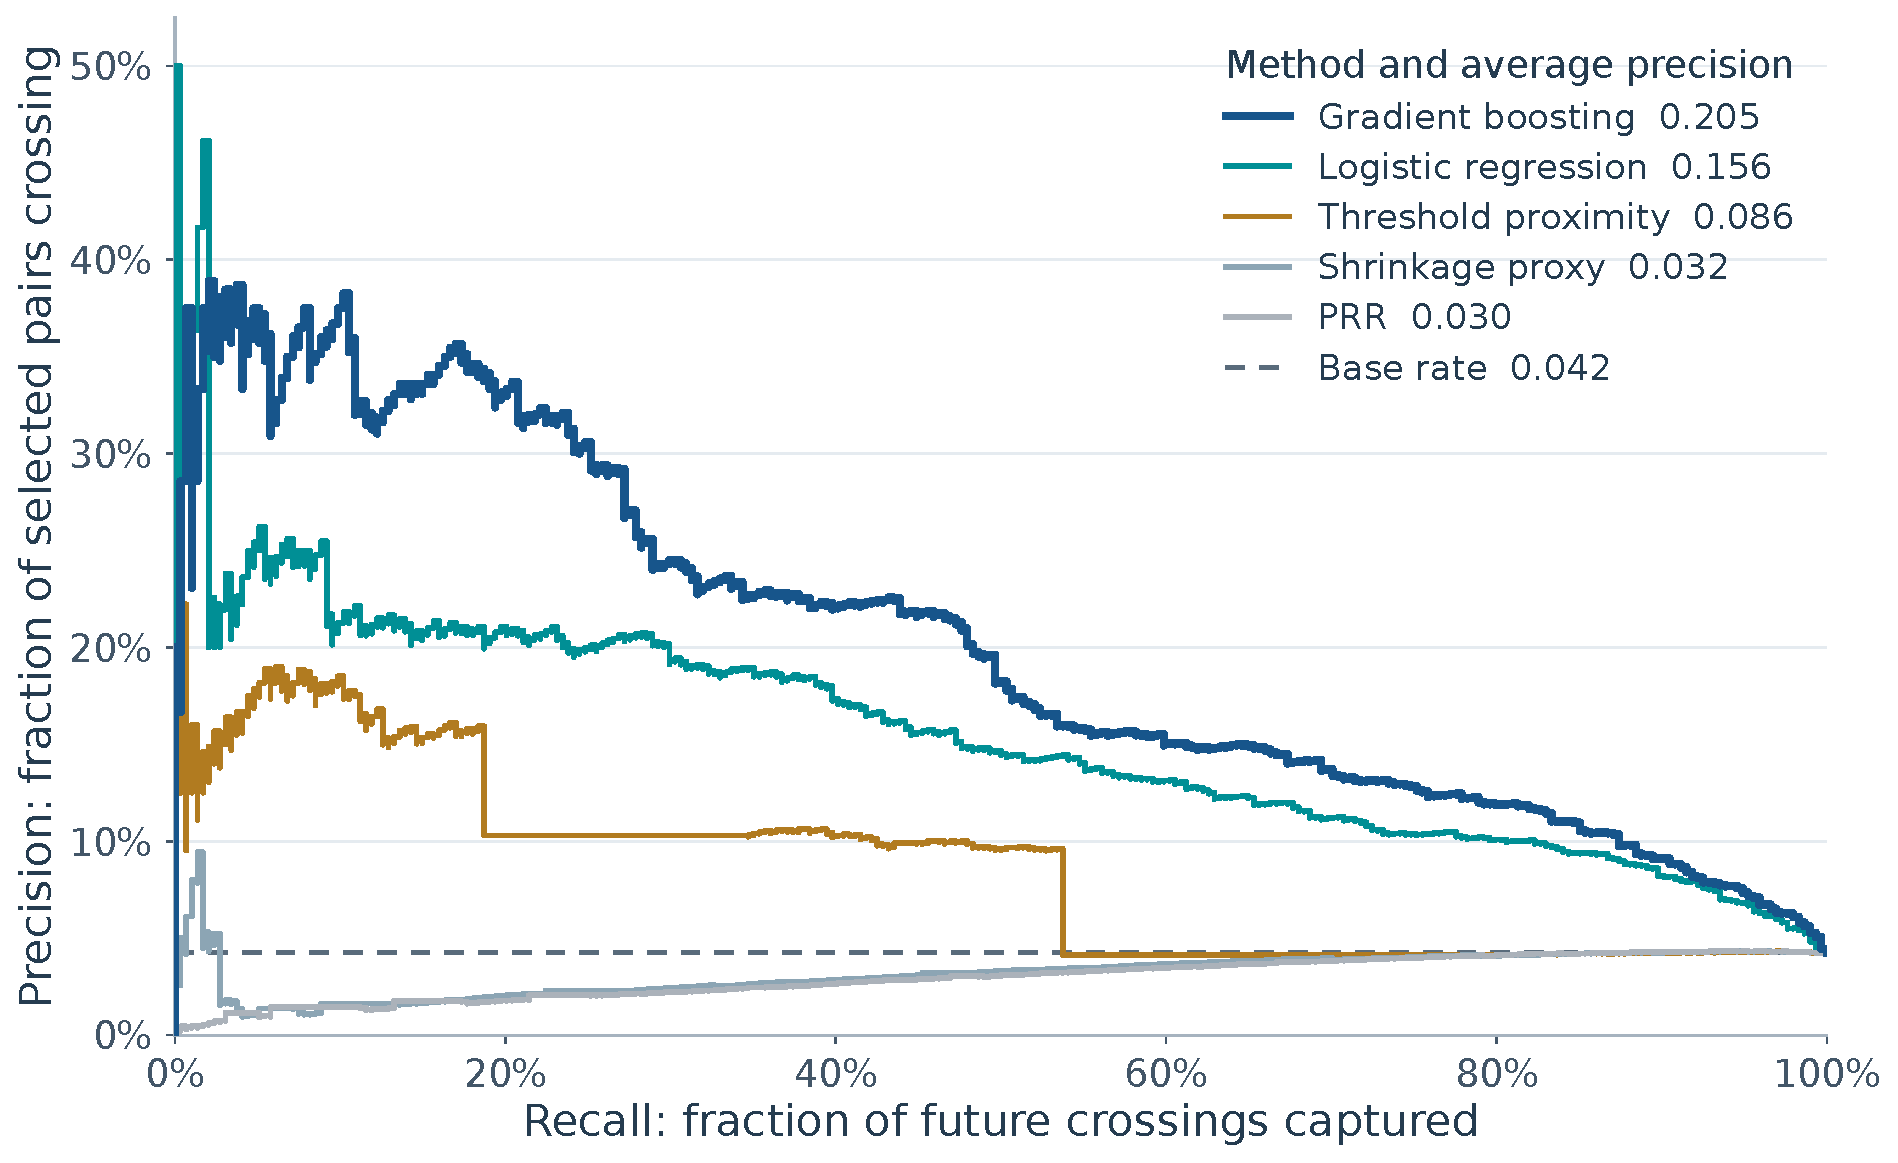
\includegraphics[width=\linewidth,height=19.6cm,keepaspectratio]{poster_figures/poster_precision_recall.pdf}
\par\vspace{0.15cm}\RaggedRight
{\captionfont Gradient boosting AP: \textbf{\GBAP}. Descriptive 95\% row-bootstrap interval: \textbf{\CIlo--\CIhi} (200 resamples).}
\end{posterbox}
\end{textblock*}

\begin{textblock*}{28.68cm}(31.38cm,54.2cm)
\begin{posterbox}{47.4cm}{Fewer reviews for the same capture}
\centering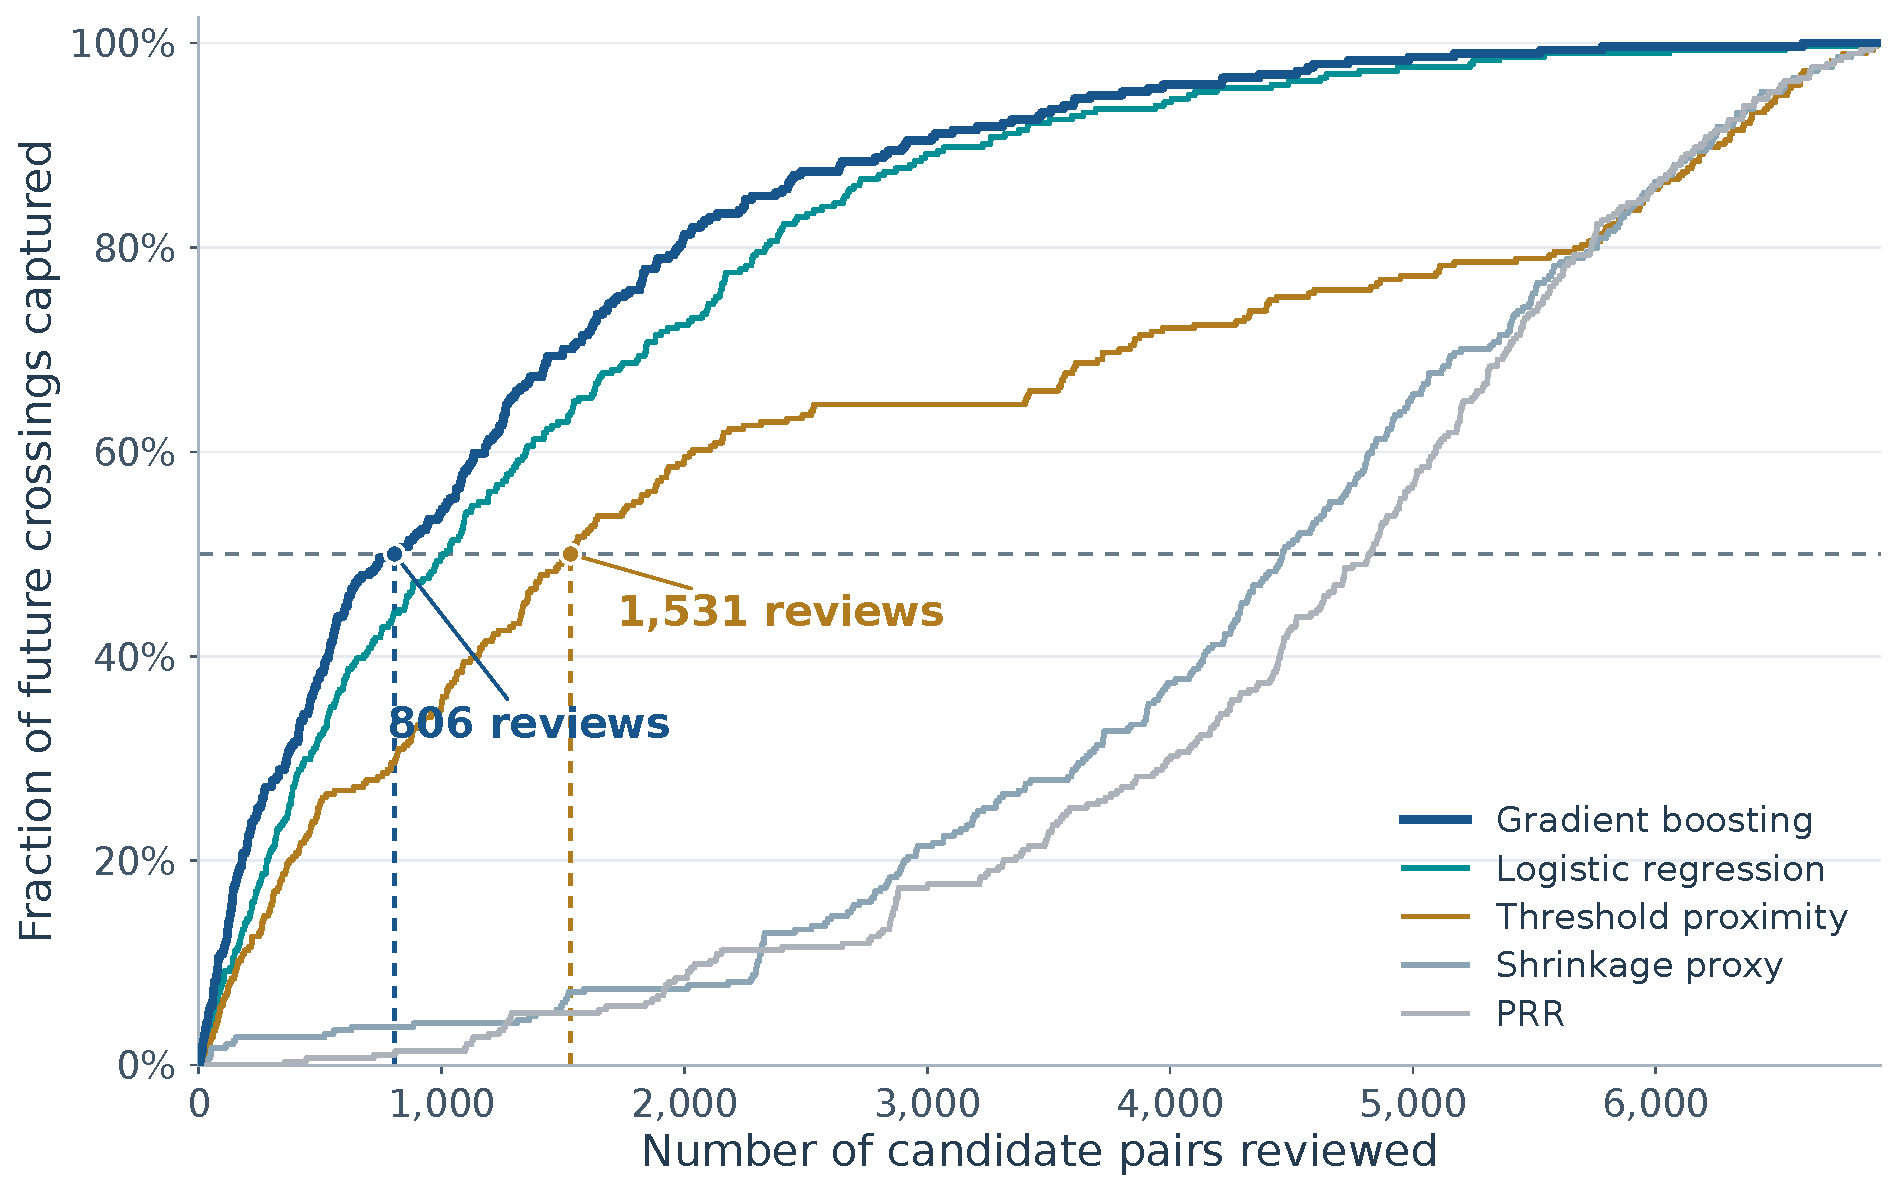
\includegraphics[width=\linewidth,height=20.7cm,keepaspectratio]{poster_figures/poster_review_efficiency.pdf}
\par\vspace{0.3cm}\RaggedRight
{\fontsize{28}{35}\selectfont\renewcommand{\arraystretch}{1.30}\setlength{\tabcolsep}{12pt}
\begin{tabularx}{\linewidth}{@{}>{\raggedright\arraybackslash}Xrr@{}}
\toprule
\textbf{Target captured} & \textbf{50\%} & \textbf{80\%}\\
\midrule
Gradient boosting & \ReviewsGB & \GBEighty\\
Threshold proximity & \ReviewsBaseline & \BaselineEighty\\
\textbf{Reduction in reviews} & \textbf{\Reduction} & \textbf{\ReductionEighty}\\
\bottomrule
\end{tabularx}}
\par\vspace{0.5cm}
\textbf{\FewerReviews\ fewer pairs} need review to capture half of the eligible future crossings.
\spacepara
{\captionfont Counts assume equal review effort per pair. They do not measure staff hours, cost savings, or clinical benefit.}
\end{posterbox}
\end{textblock*}

% ---------------- RIGHT COLUMN ----------------
\begin{textblock*}{28.68cm}(61.16cm,20.4cm)
\begin{posterbox}{18.5cm}{Most crossings are returning signals}
\begin{minipage}[t]{0.49\linewidth}
{\fontsize{54}{63}\selectfont\bfseries\color{Blue}245 / 294}\par\vspace{.25cm}
{\smallbody\textbf{83.3\%} had been strong in an earlier quarter.}
\end{minipage}\hfill
\begin{minipage}[t]{0.44\linewidth}
{\fontsize{54}{63}\selectfont\bfseries\color{Teal}49}\par\vspace{.25cm}
{\smallbody had no earlier strong quarter in the available history.}
\end{minipage}
\spacepara
{\captionfont History starts in 2022. Eligibility excludes pairs strong \emph{now}; earlier strong quarters are allowed. The endpoint includes recurrence.}
\end{posterbox}
\end{textblock*}

\begin{textblock*}{28.68cm}(61.16cm,40.4cm)
\begin{posterbox}{23.5cm}{Performance across nine test quarters}
\centering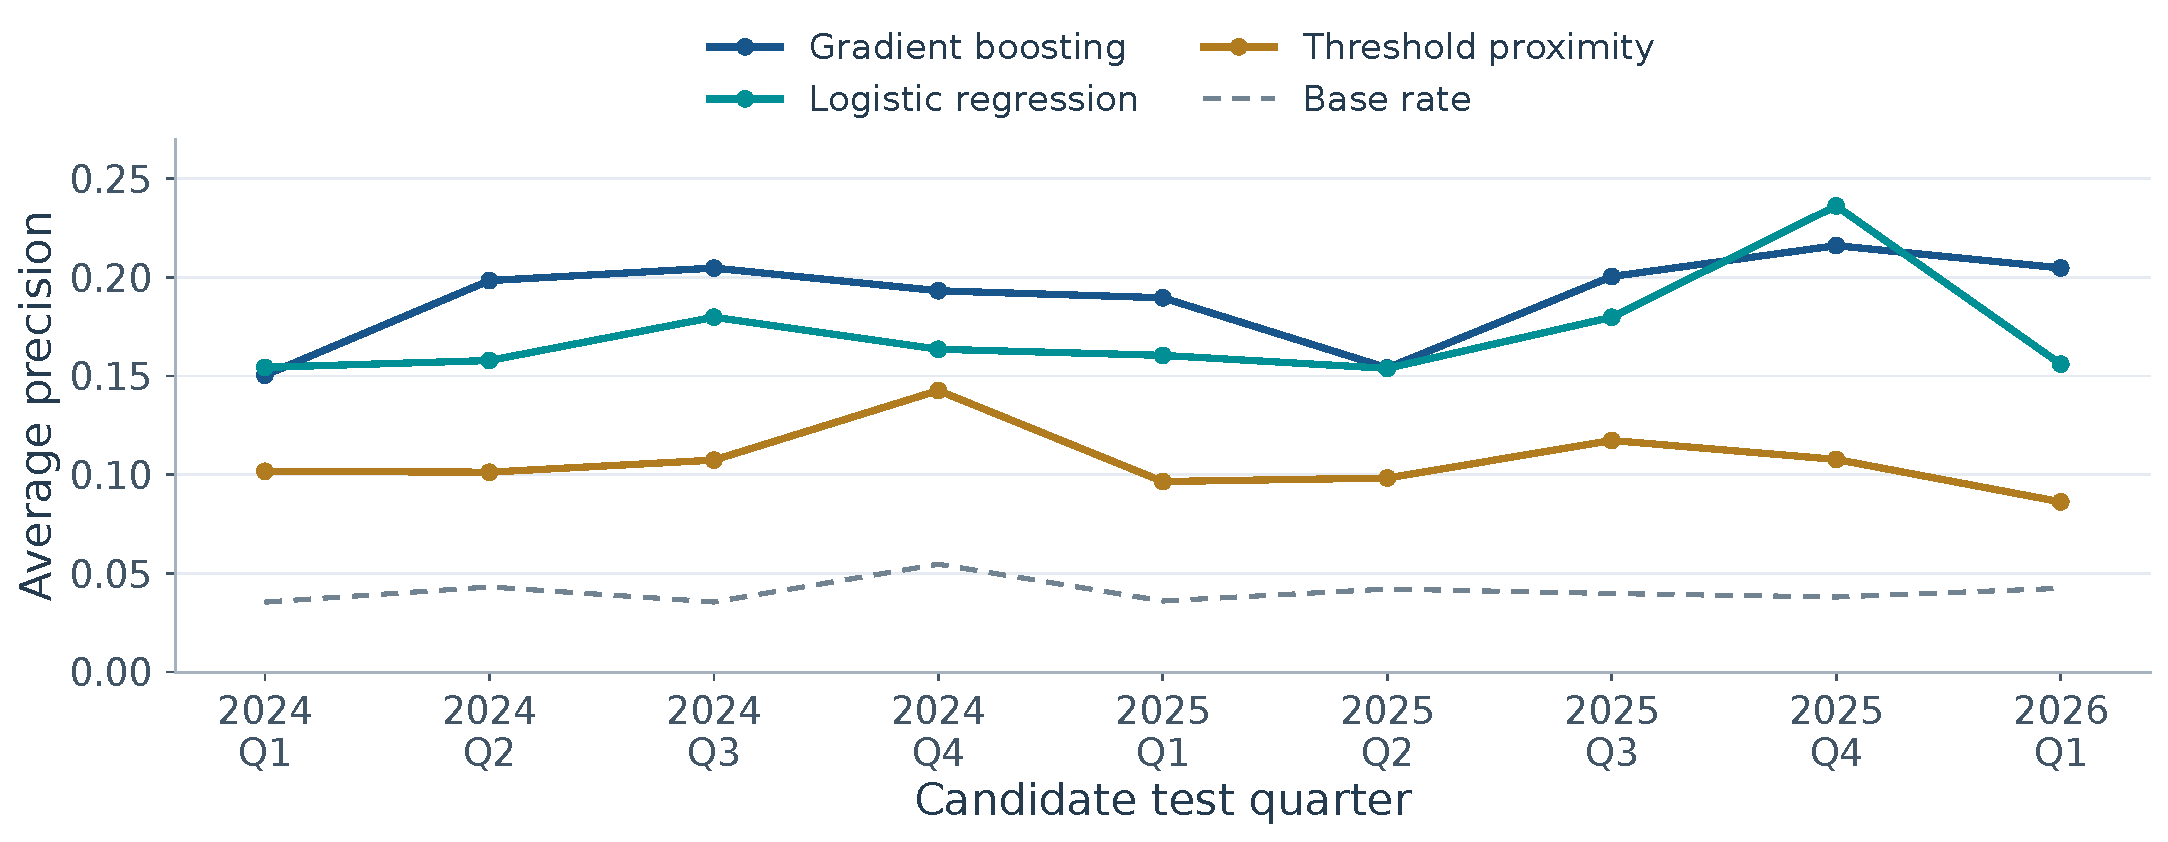
\includegraphics[width=\linewidth]{poster_figures/poster_rolling_validation.pdf}
\par\vspace{0.15cm}\RaggedRight
{\captionfont Both fitted models exceeded threshold proximity in all nine quarters. Logistic regression led in 2024Q1 and 2025Q4.}
\end{posterbox}
\end{textblock*}

\begin{textblock*}{28.68cm}(61.16cm,65.4cm)
\begin{posterbox}{18.8cm}{Recent history adds predictive value}
\centering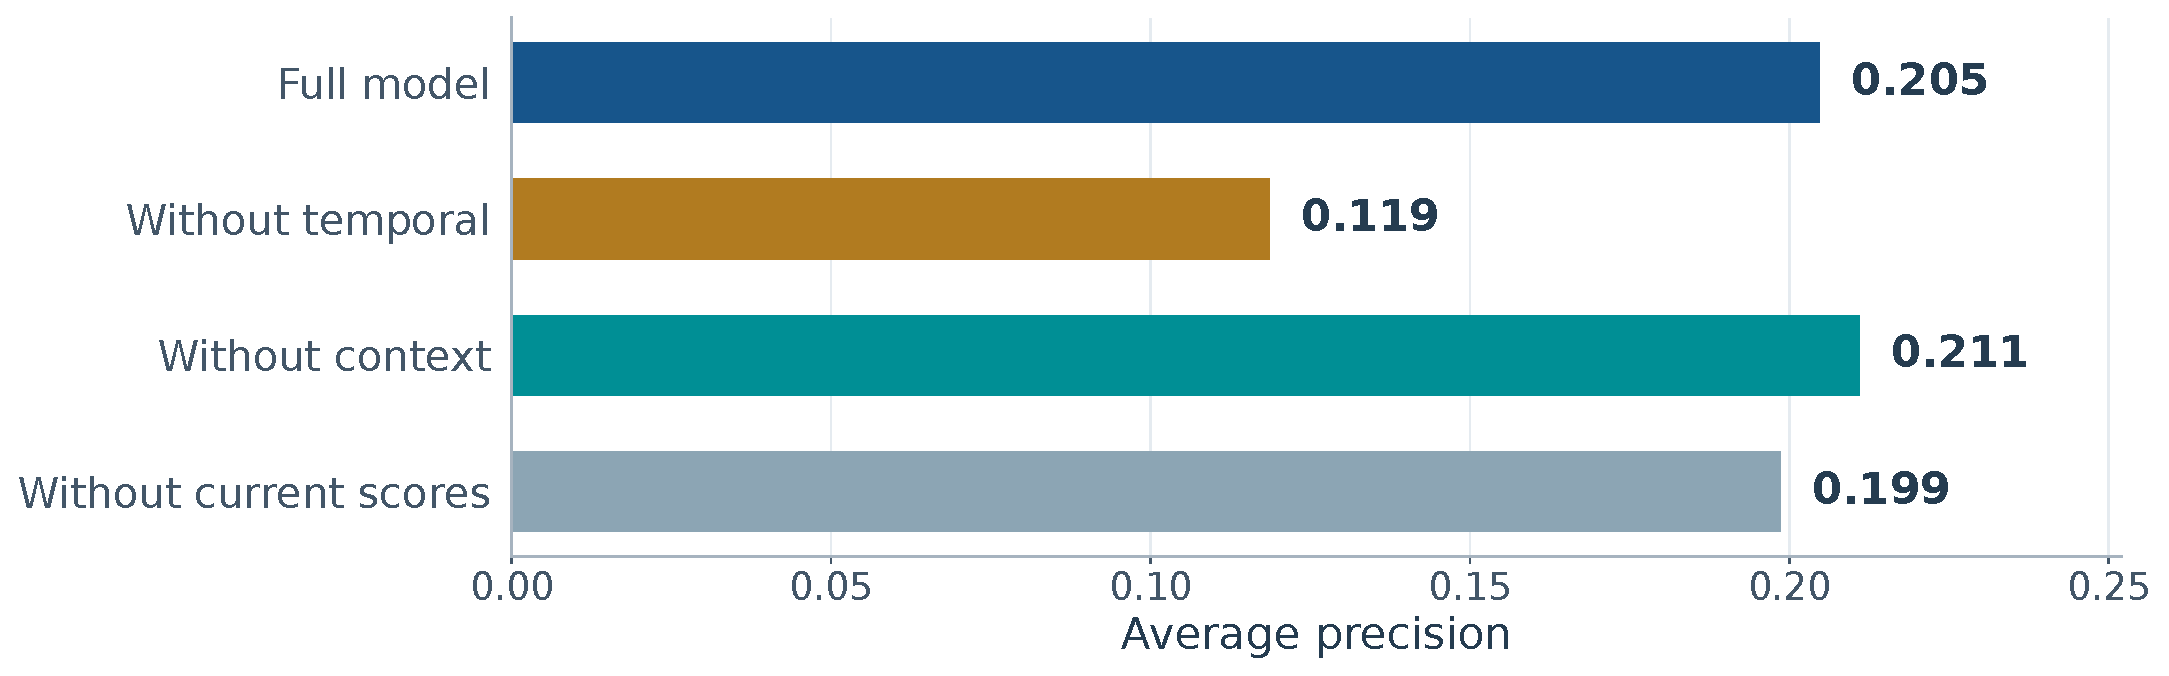
\includegraphics[width=\linewidth]{poster_figures/poster_ablation.pdf}
\par\vspace{0.15cm}\RaggedRight
{\captionfont Removing temporal features lowered AP to \textbf{\NoTemporalAP}. Omitting context did not lower AP.}
\end{posterbox}
\end{textblock*}

\begin{textblock*}{28.68cm}(61.16cm,85.7cm)
\begin{posterbox}{15.9cm}{Interpretation and limits}
\smallbody
\textbf{The ranking enriches a queue for expert review.} Outcomes are statistical proxy crossings. Passive VAERS reports establish neither incidence nor vaccine causality.
\spacepara
Public-data availability lags limit real-time claims. Pairs share reports, so row-bootstrap intervals are descriptive. Clinical usefulness requires expert validation.
\end{posterbox}
\end{textblock*}

% Compact reference and contact strip; no unsupported clinical claims.
\begin{textblock*}{68.5cm}(1.6cm,103.55cm)
{\fontsize{24}{29}\selectfont\bfseries\color{Navy}AIPM 2026}\hspace{0.6cm}%
{\fontsize{21}{27}\selectfont\color{Muted}Data: U.S. VAERS public files, 2022--2026. Analysis restricted to receipt quarters through 2026Q2.}
\par\vspace{0.19cm}
{\fontsize{19}{25}\selectfont\color{Muted}
\textbf{References:} Evans et al. \emph{Pharmacoepidemiol Drug Saf.} 2001;10:483--486. \href{https://doi.org/10.1002/pds.677}{doi:10.1002/pds.677}.
Bate et al. \emph{Eur J Clin Pharmacol.} 1998;54:315--321. \href{https://doi.org/10.1007/s002280050466}{doi:10.1007/s002280050466}.
\href{https://vaers.hhs.gov/data/dataguide.html}{VAERS data guidance}.}
\end{textblock*}
\begin{textblock*}{18.5cm}(71.34cm,103.6cm)
\begin{minipage}[c]{14.7cm}
\raggedleft
{\fontsize{24}{29}\selectfont\color{Navy}\bfseries Contact}\par
{\fontsize{23}{28}\selectfont\href{mailto:nalpay@uci.edu}{nalpay@uci.edu}}\par
{\fontsize{19}{24}\selectfont\color{Muted}\href{https://alpaynatanael.github.io/index.html}{Website / QR}}
\end{minipage}\hfill
\begin{minipage}[c]{2.5cm}
\qrcode[height=2.2cm]{https://alpaynatanael.github.io/index.html}
\end{minipage}
\end{textblock*}
\null
\end{document}
